\subsubsection{pr11}
\label{subsubsec:pr11}
The obtained results were the following:
{
\renewcommand{\arraystretch}{2}
\begin{longtable}[h]{| c | c | c | c | c |}
    \hline
    \textbf{Failures} & \multicolumn{3}{c}{Time limit} & \\
    \hline
    \textbf{Search strategy} & \textbf{\textit{30 sec}} & \textbf{\textit{1 min}} & \textbf{\textit{2 min}} & \textbf{\textit{5 min}} \\
    \hline
    \endhead
    default search                                         &  81.602 & 195.823 & 434.744 & 1.111.163 \\
    \hline
    domWdeg, random                                        & 100.422 & 228.389 & 456.151 & 1.138.595 \\
    \hline
    \textit{domWdeg, random, Luby restart L=250}           &  52.859 & 113.525 & 260.911 &  678.802 \\
    \hline
    \textit{domWdeg, random, Luby restart L=250, LNS 85\%} &   2.001 &  15.047 & 148.494 &  755.877 \\
    \hline
    domWdeg, random, Luby restart L=250, LNS 15\%          &  71.388 & 152.697 & 344.690 &  883.169 \\
    \hline
    first fail, min                                        &  34.099 & 103.978 & 305.211 & 1.014.646 \\
    \hline
\end{longtable}
}
\begin{figure}[H]
    \centering
    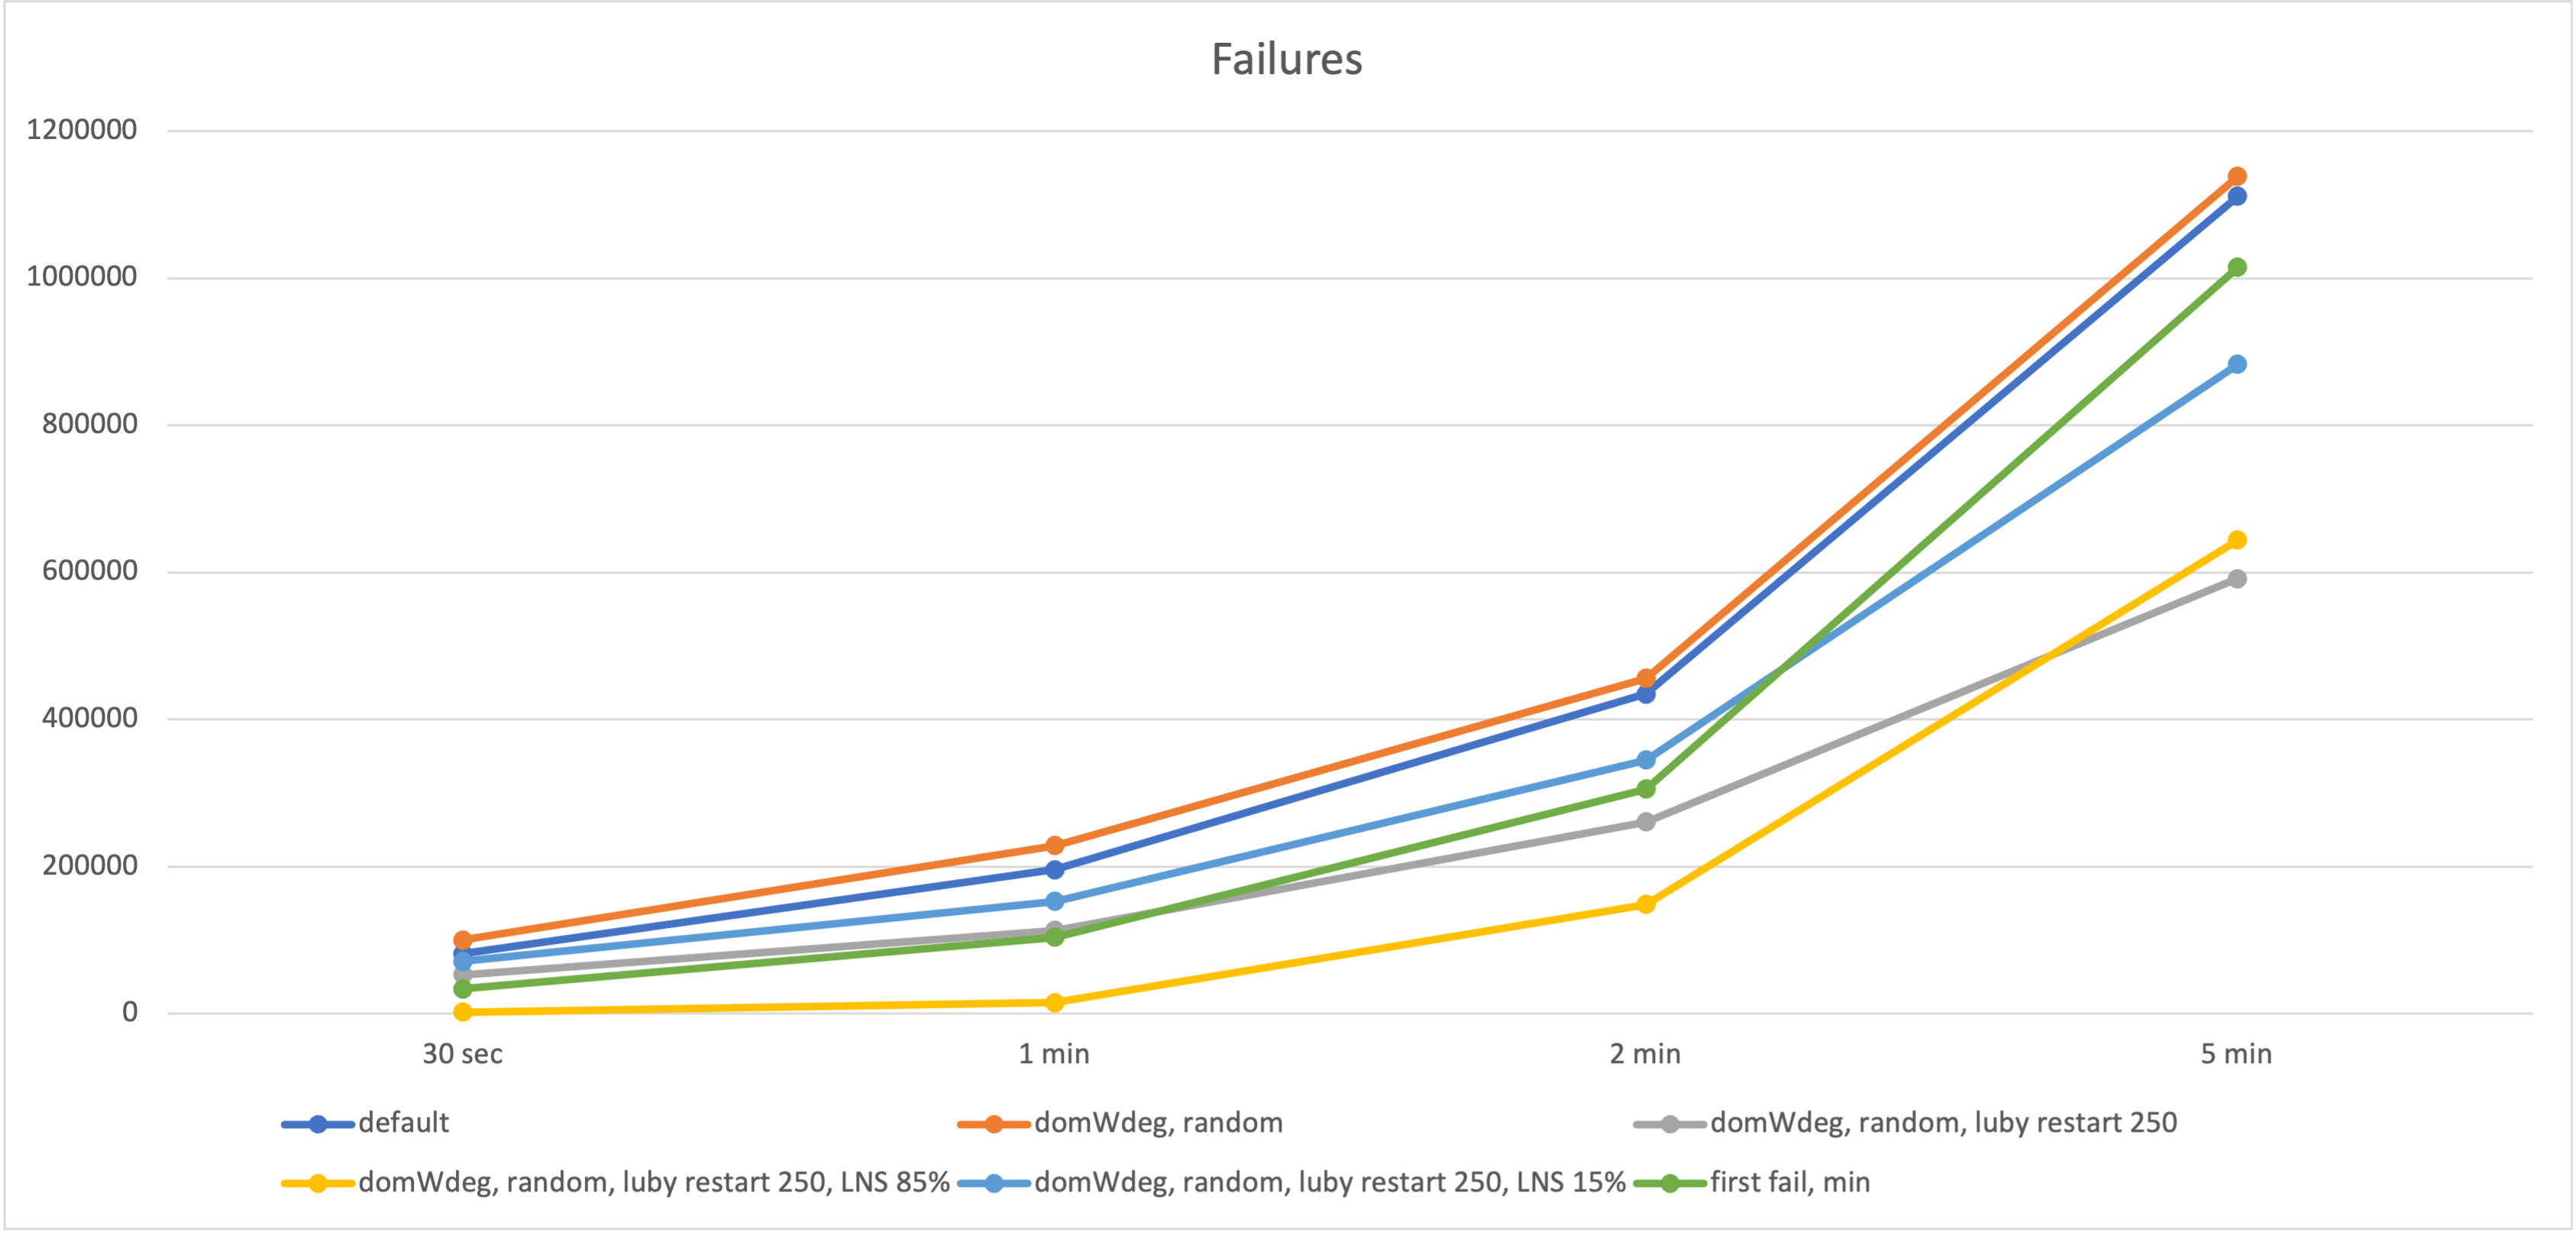
\includegraphics[width=0.8\columnwidth]{../graphs/pr11-failures.png}
    \caption{Failures graph for \textbf{pr11}.}
\end{figure}

{
\renewcommand{\arraystretch}{2}
\begin{longtable}[h]{| c | c | c | c | c |}
    \hline
    \textbf{Objective function} & \multicolumn{3}{c}{Time limit} & \\
    \hline
    \textbf{Search strategy} & \textbf{\textit{30 sec}} & \textbf{\textit{1 min}} & \textbf{\textit{2 min}} & \textbf{\textit{5 min}} \\
    \hline
    \endhead
    default search                                         & 25.406.700 & 25.256.890 & 25.066.060 & 25.066.060 \\
    \hline
    domWdeg, random                                        & 33.163.620 & 33.163.620 & 32.477.780 & 31.217.300 \\
    \hline
    domWdeg, random, Luby restart L=250                    & 31.640.290 & 31.640.290 & 31.125.930 & 29.831.450 \\
    \hline
    \textit{domWdeg, random, Luby restart L=250, LNS 85\%} & 20.251.920 & 13.628.410 & 10.521.670 & 10.087.210 \\
    \hline
    domWdeg, random, Luby restart L=250, LNS 15\%          & 28.391.400 & 27.467.130 & 27.303.410 & 27.226.400 \\
    \hline
    first fail, min                                        & 27.0354.20 & 26.796.860 & 26.066.280 & 26.066.280 \\
    \hline
\end{longtable}
}
\begin{figure}[H]
    \centering
    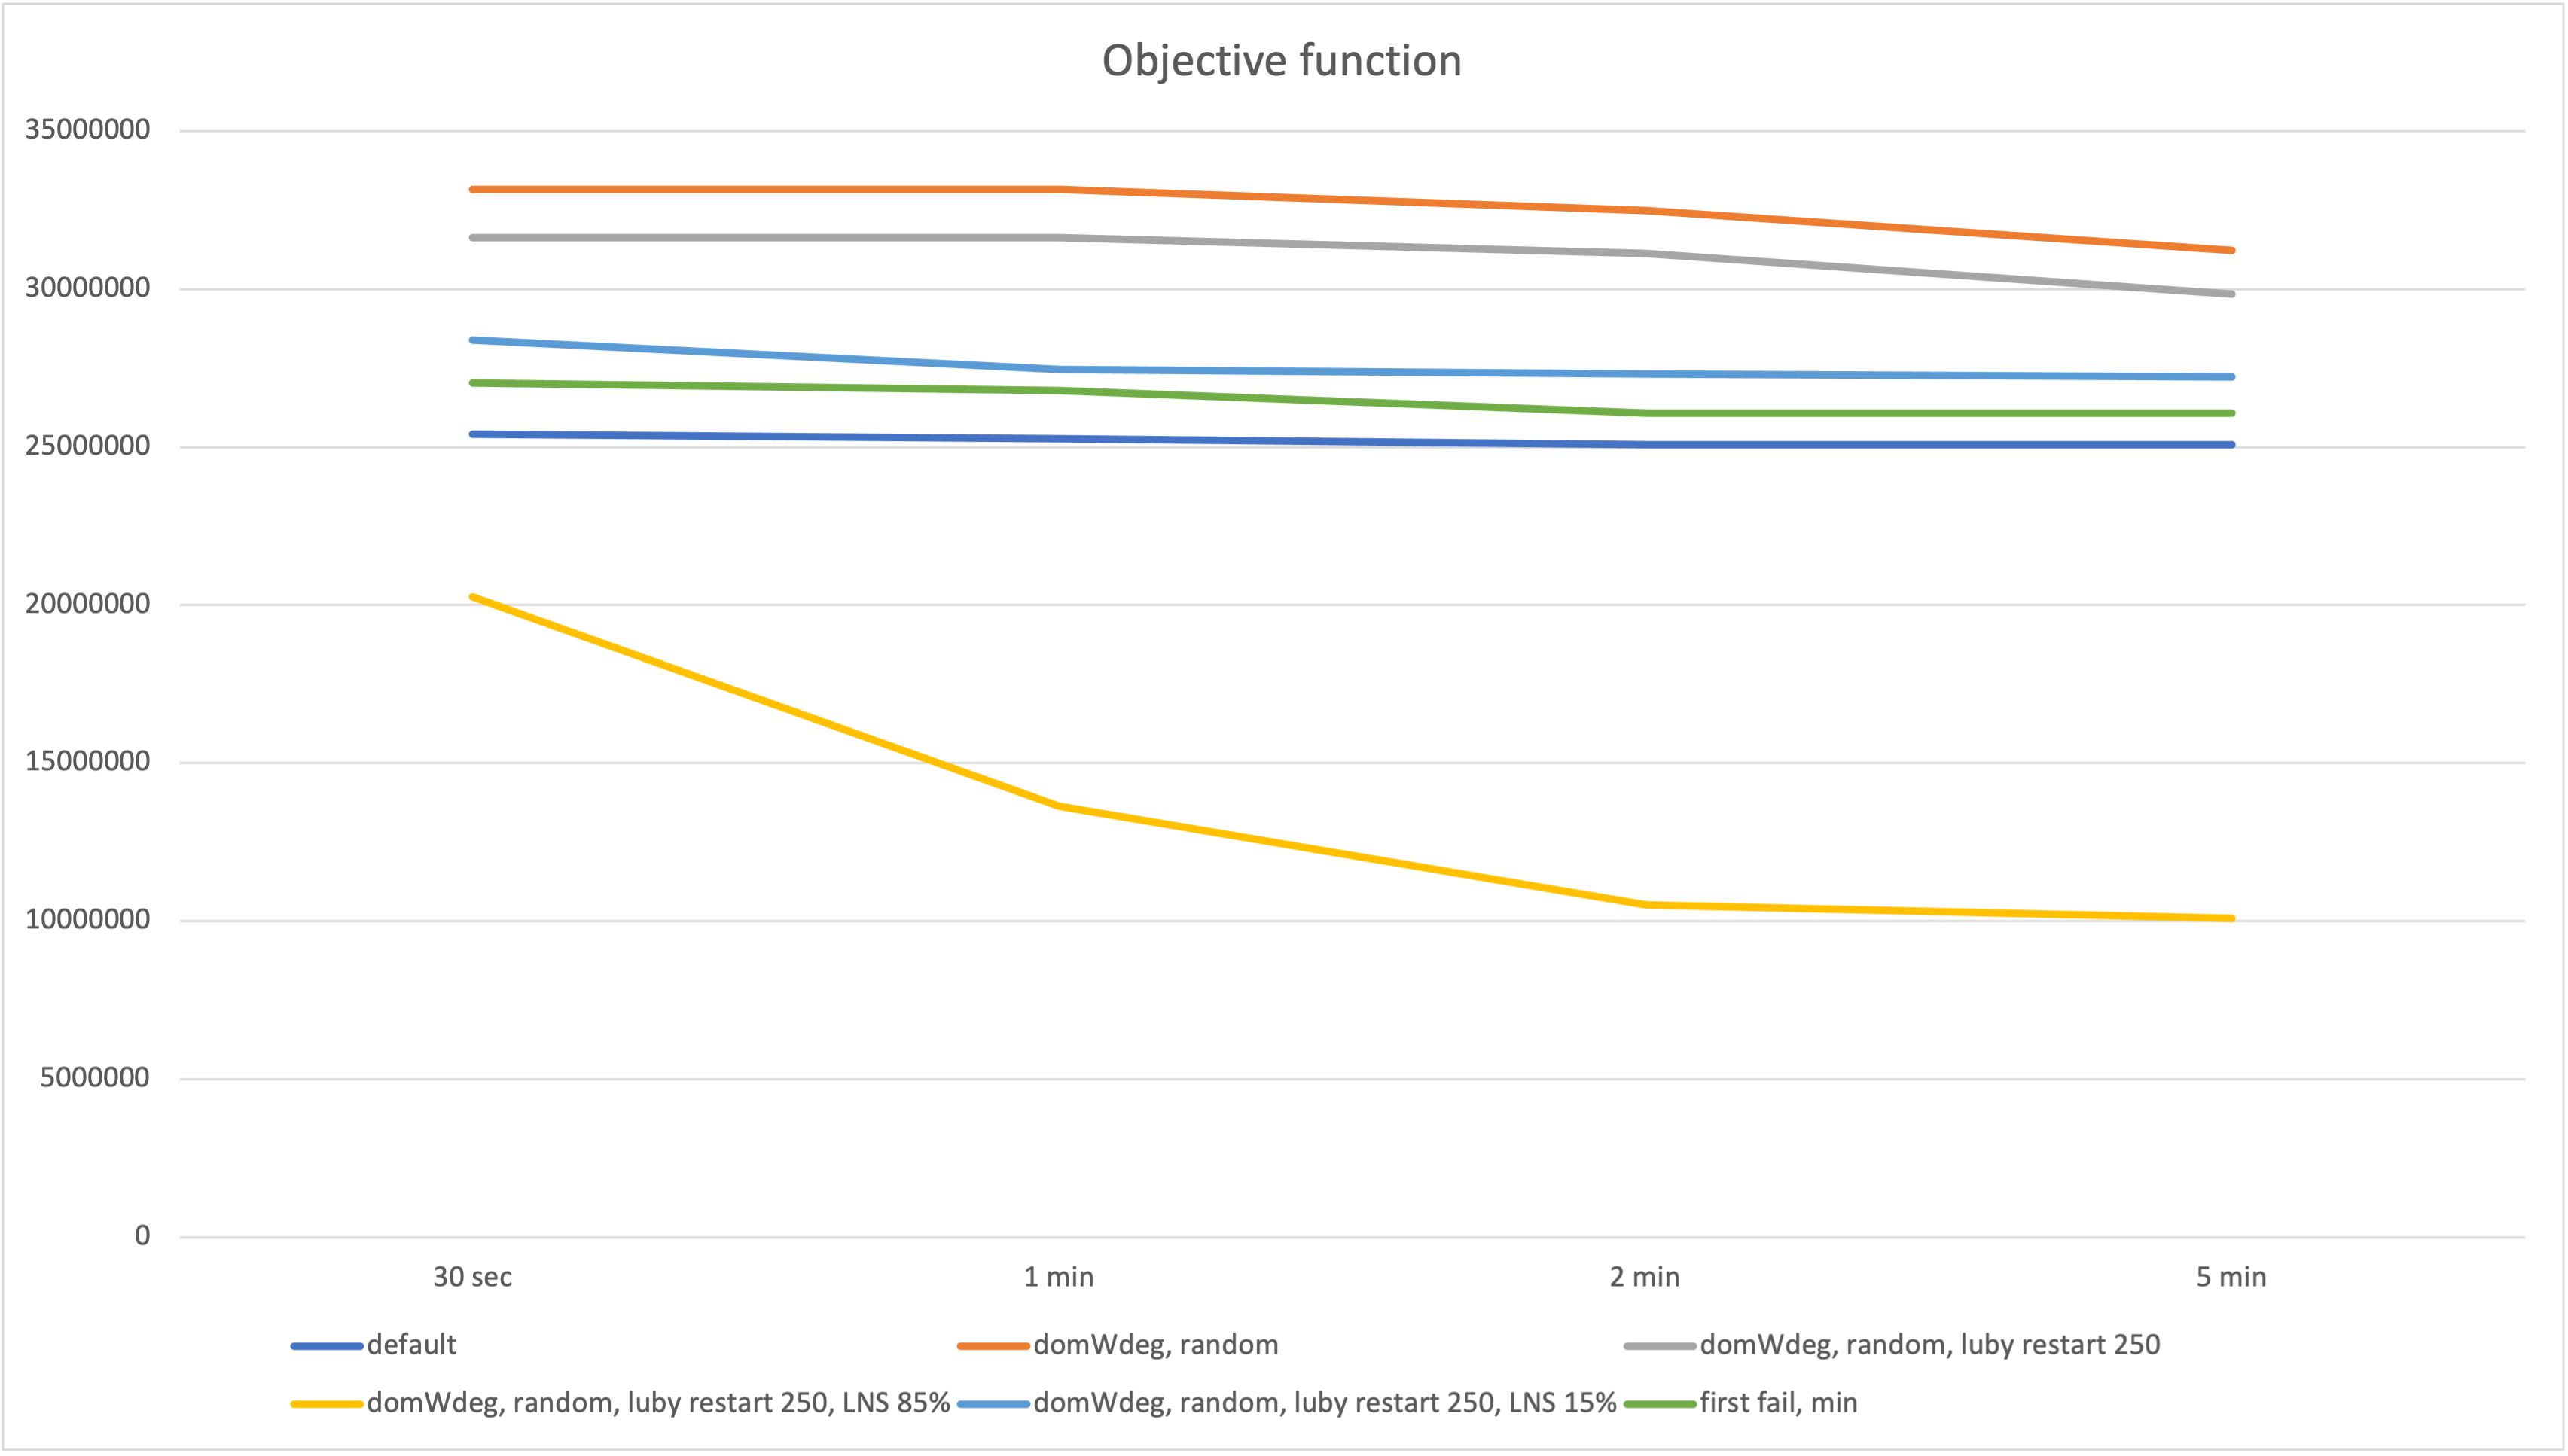
\includegraphics[width=0.8\columnwidth]{../graphs/pr11-objf.png}
    \caption{Objective functions graph for \textbf{pr11}.}
\end{figure}

{
\renewcommand{\arraystretch}{2}
\begin{longtable}[h]{| c | c | c | c |}
    \hline
    \textbf{Weights} & \textbf{Objective function} & \textbf{Total distance} & \textbf{Used vehicles} \\
    \hline
    \endhead
    $\alpha = 10, \beta = 0$ & 10.387.700 & 1.038.770 & 6 \\
    \hline
    $\alpha = 7, \beta = 3$  &  7.254.270 & 1.036.323 & 3 \\
    \hline
    $\alpha = 5, \beta = 5$  &  5.181.630 & 1.036.323 & 3 \\
    \hline
    $\alpha = 3, \beta = 7$  &  3.278.542 & 1.092.838 & 4 \\
    \hline
    $\alpha = 0, \beta = 10$ &         30 & 3.042.079 & 3 \\
    \hline
\end{longtable}
}
\begin{figure}[H]
    \centering
    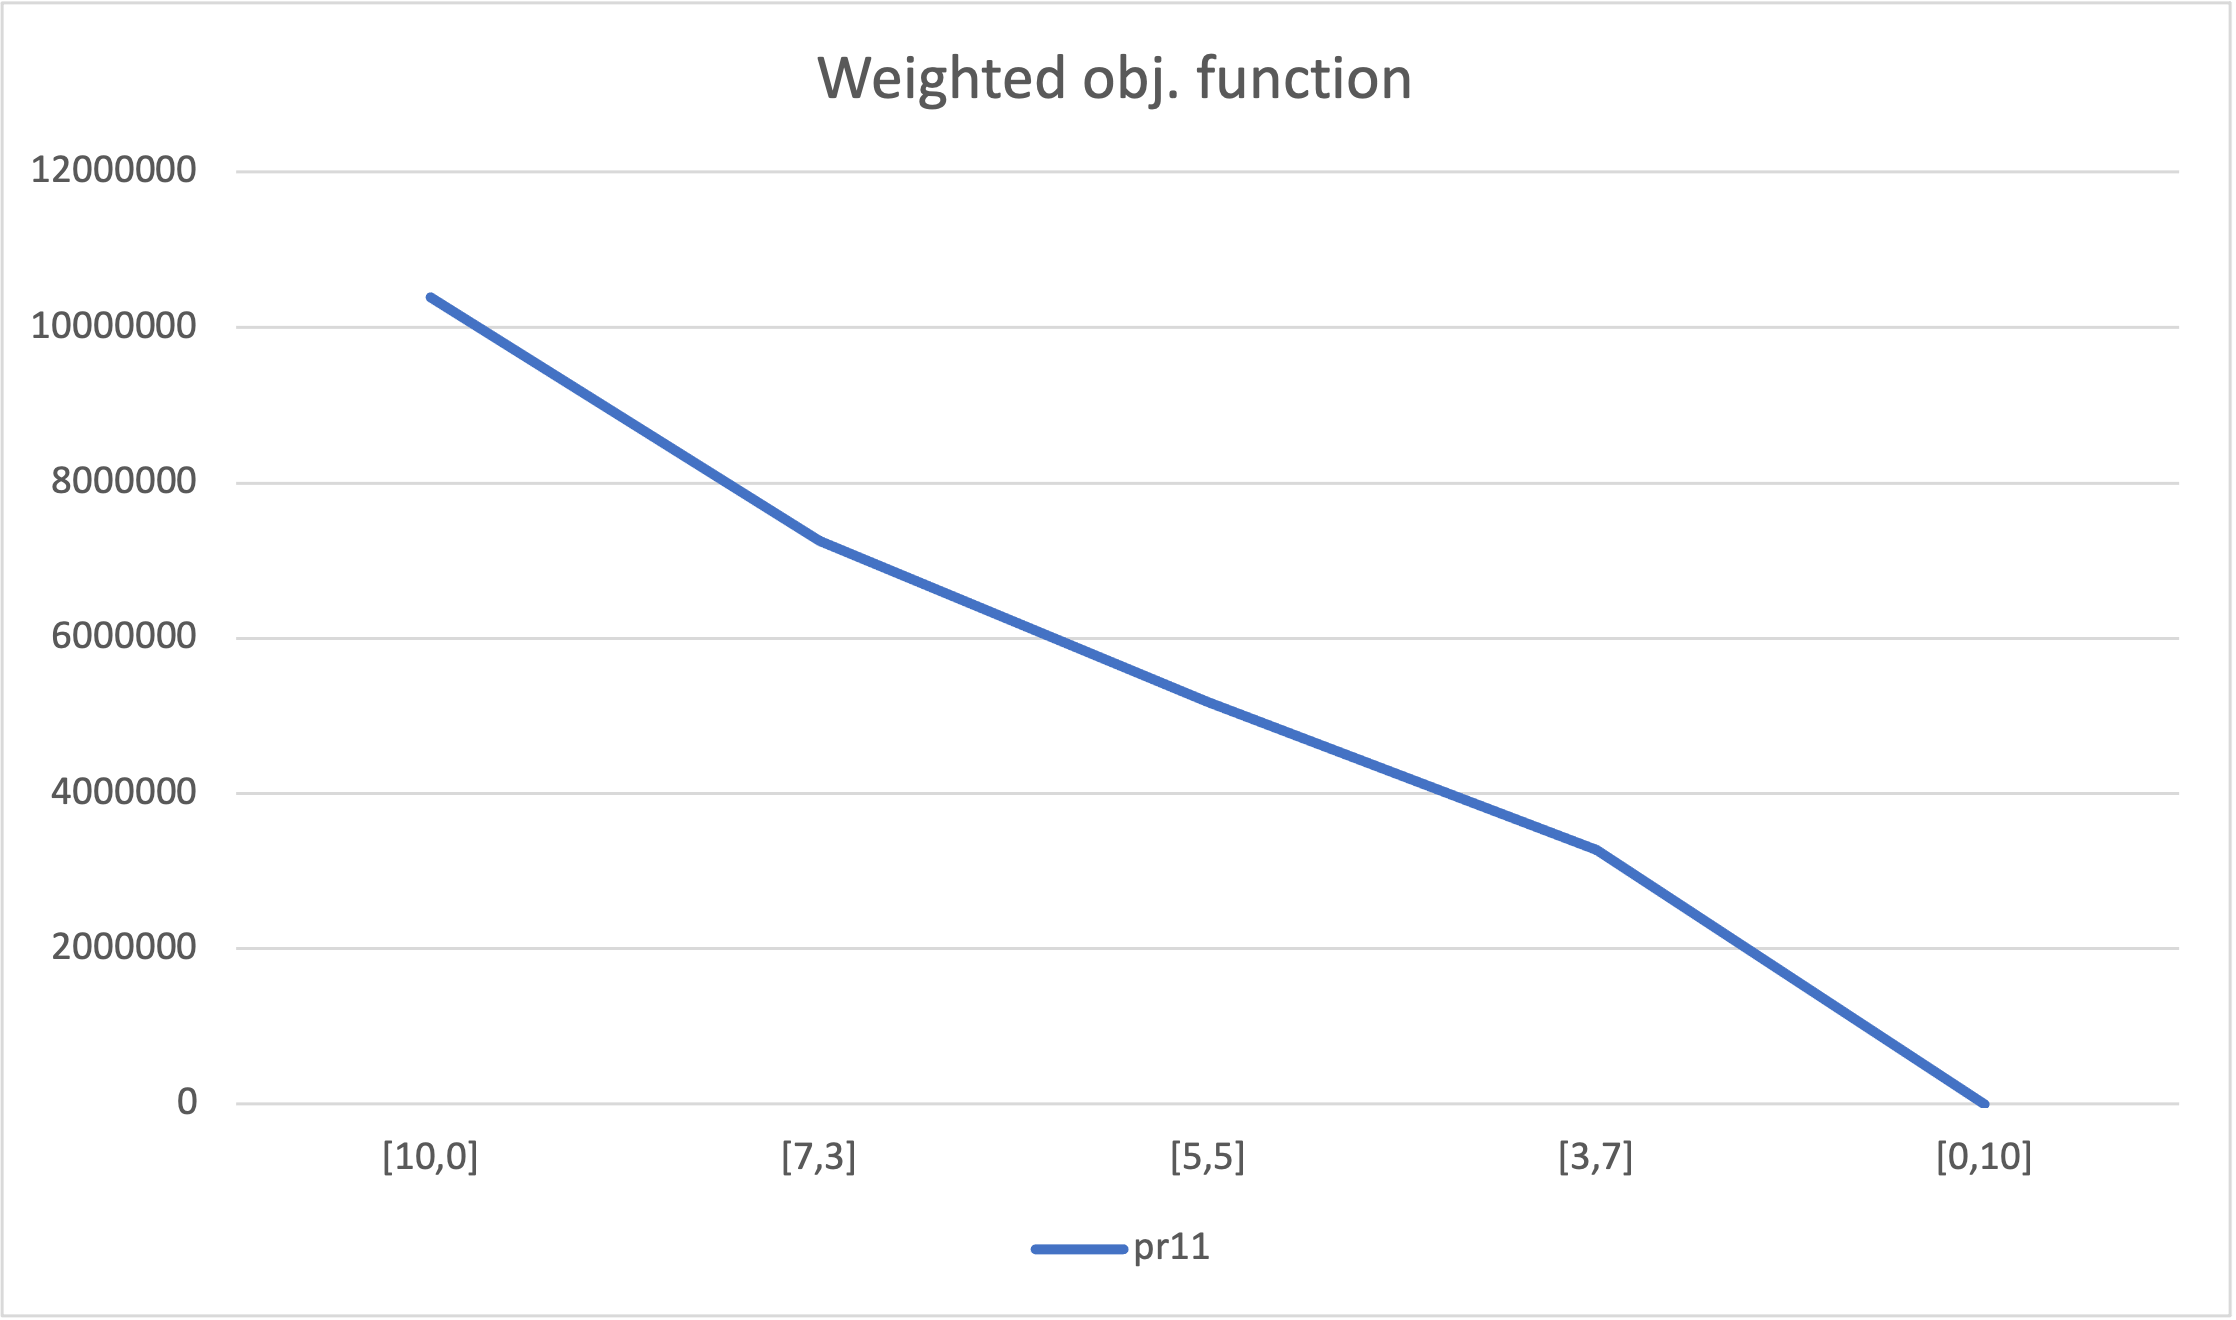
\includegraphics[height=0.25\textheight]{../graphs/pr11-wobjf.png}
    \caption{Weighted objective functions graph for \textbf{pr11}.}
\end{figure}

\begin{figure}[H]
    \centering
    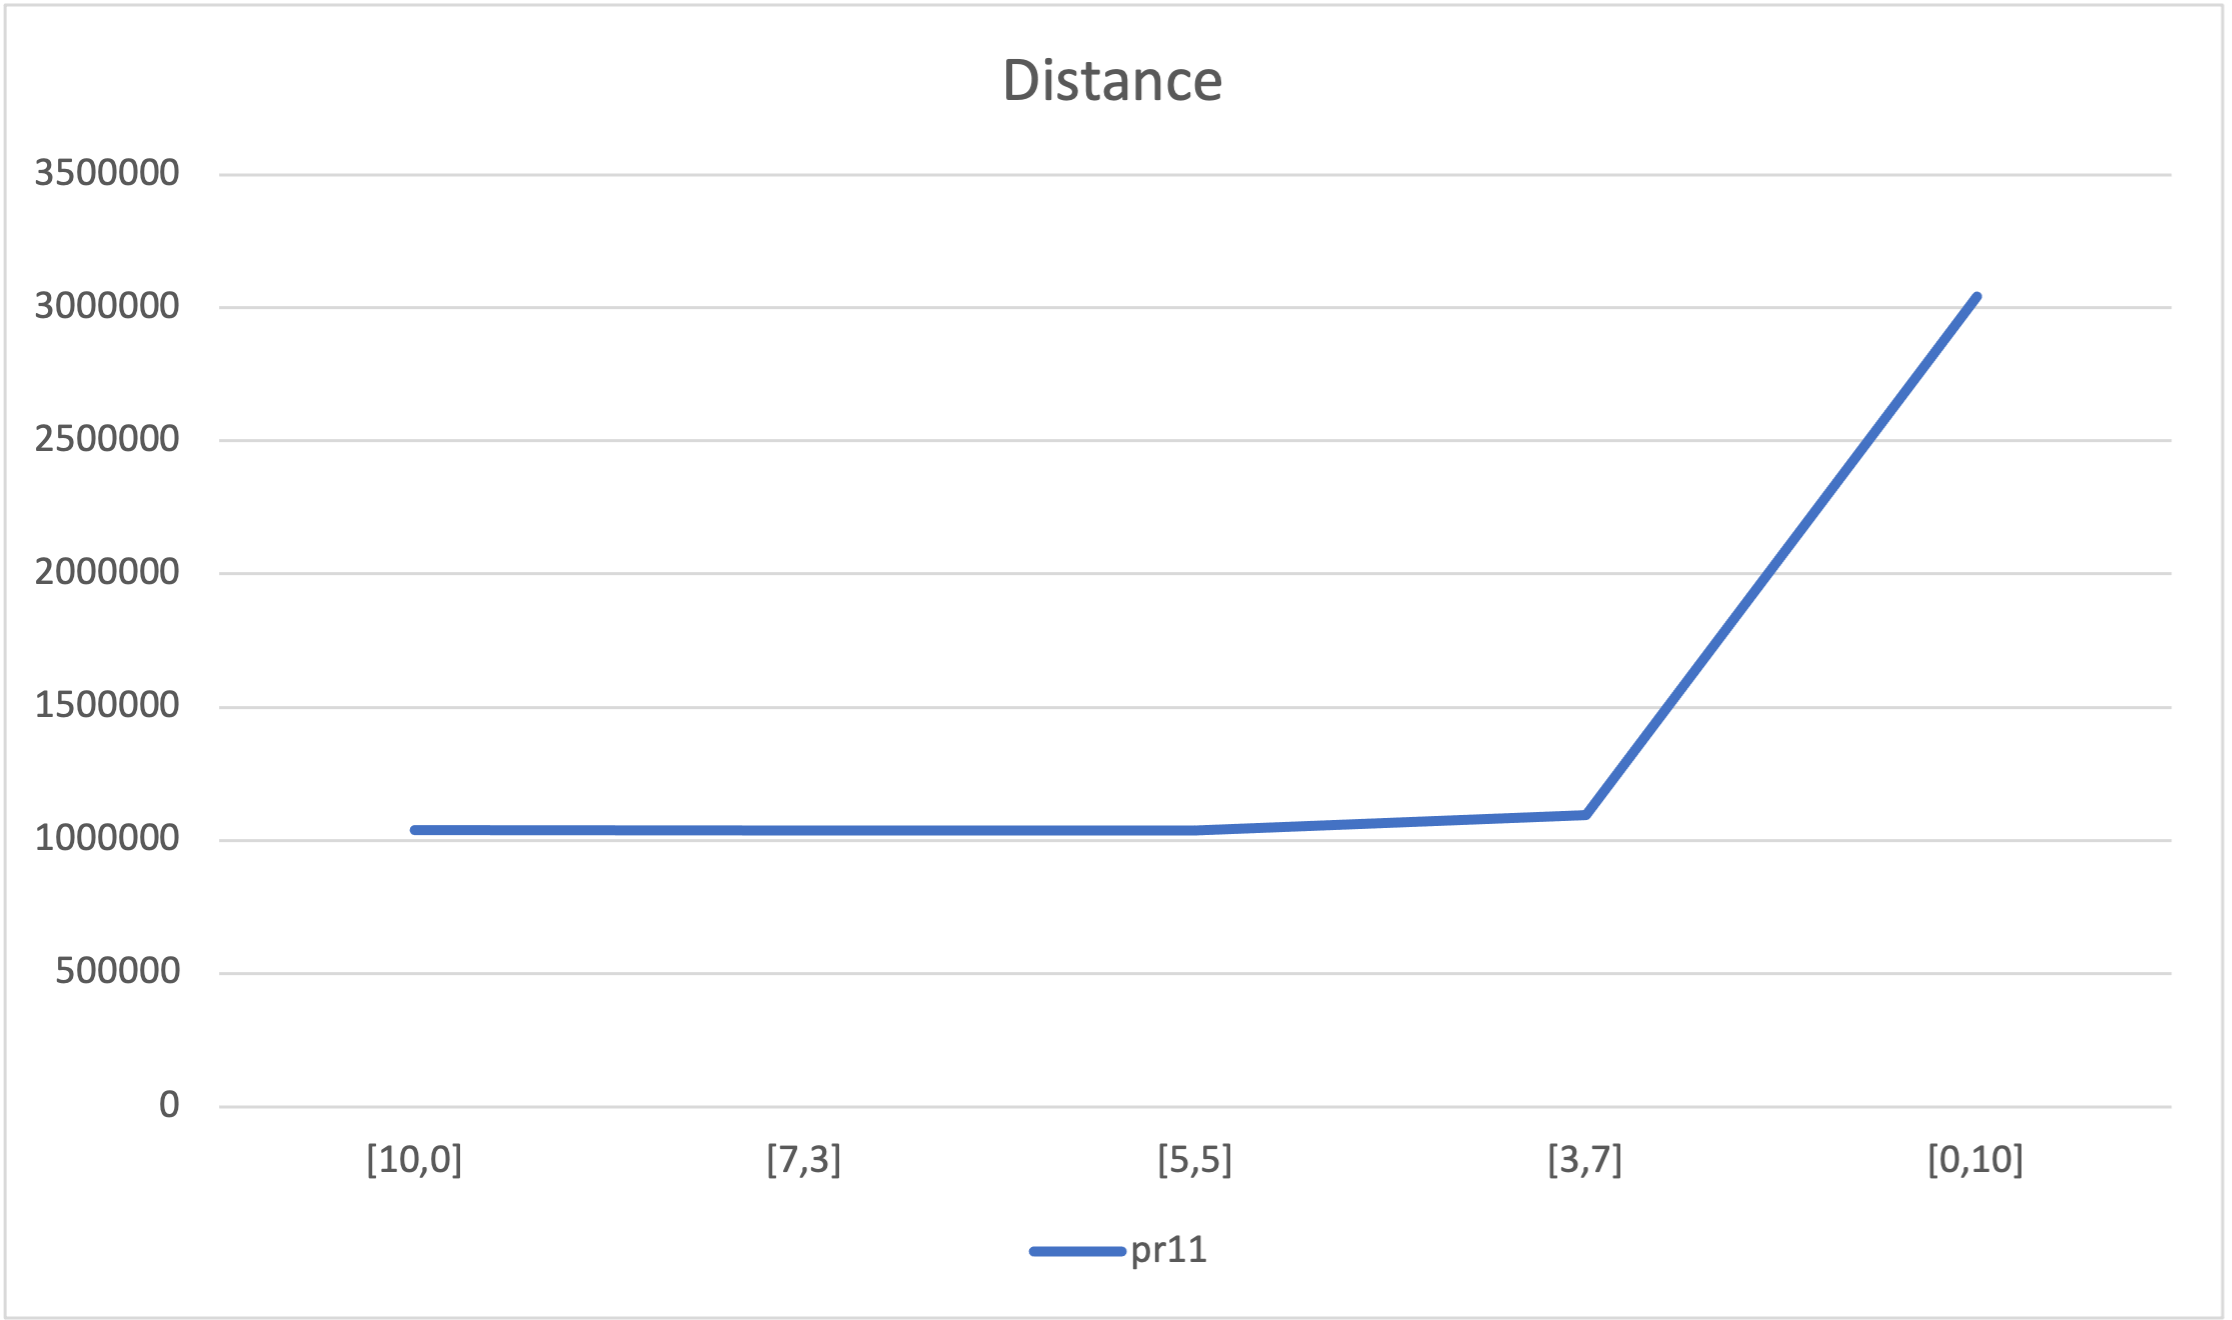
\includegraphics[height=0.25\textheight]{../graphs/pr11-distance.png}
    \caption{Distances graph for \textbf{pr11}.}
\end{figure}

\begin{figure}[H]
    \centering
    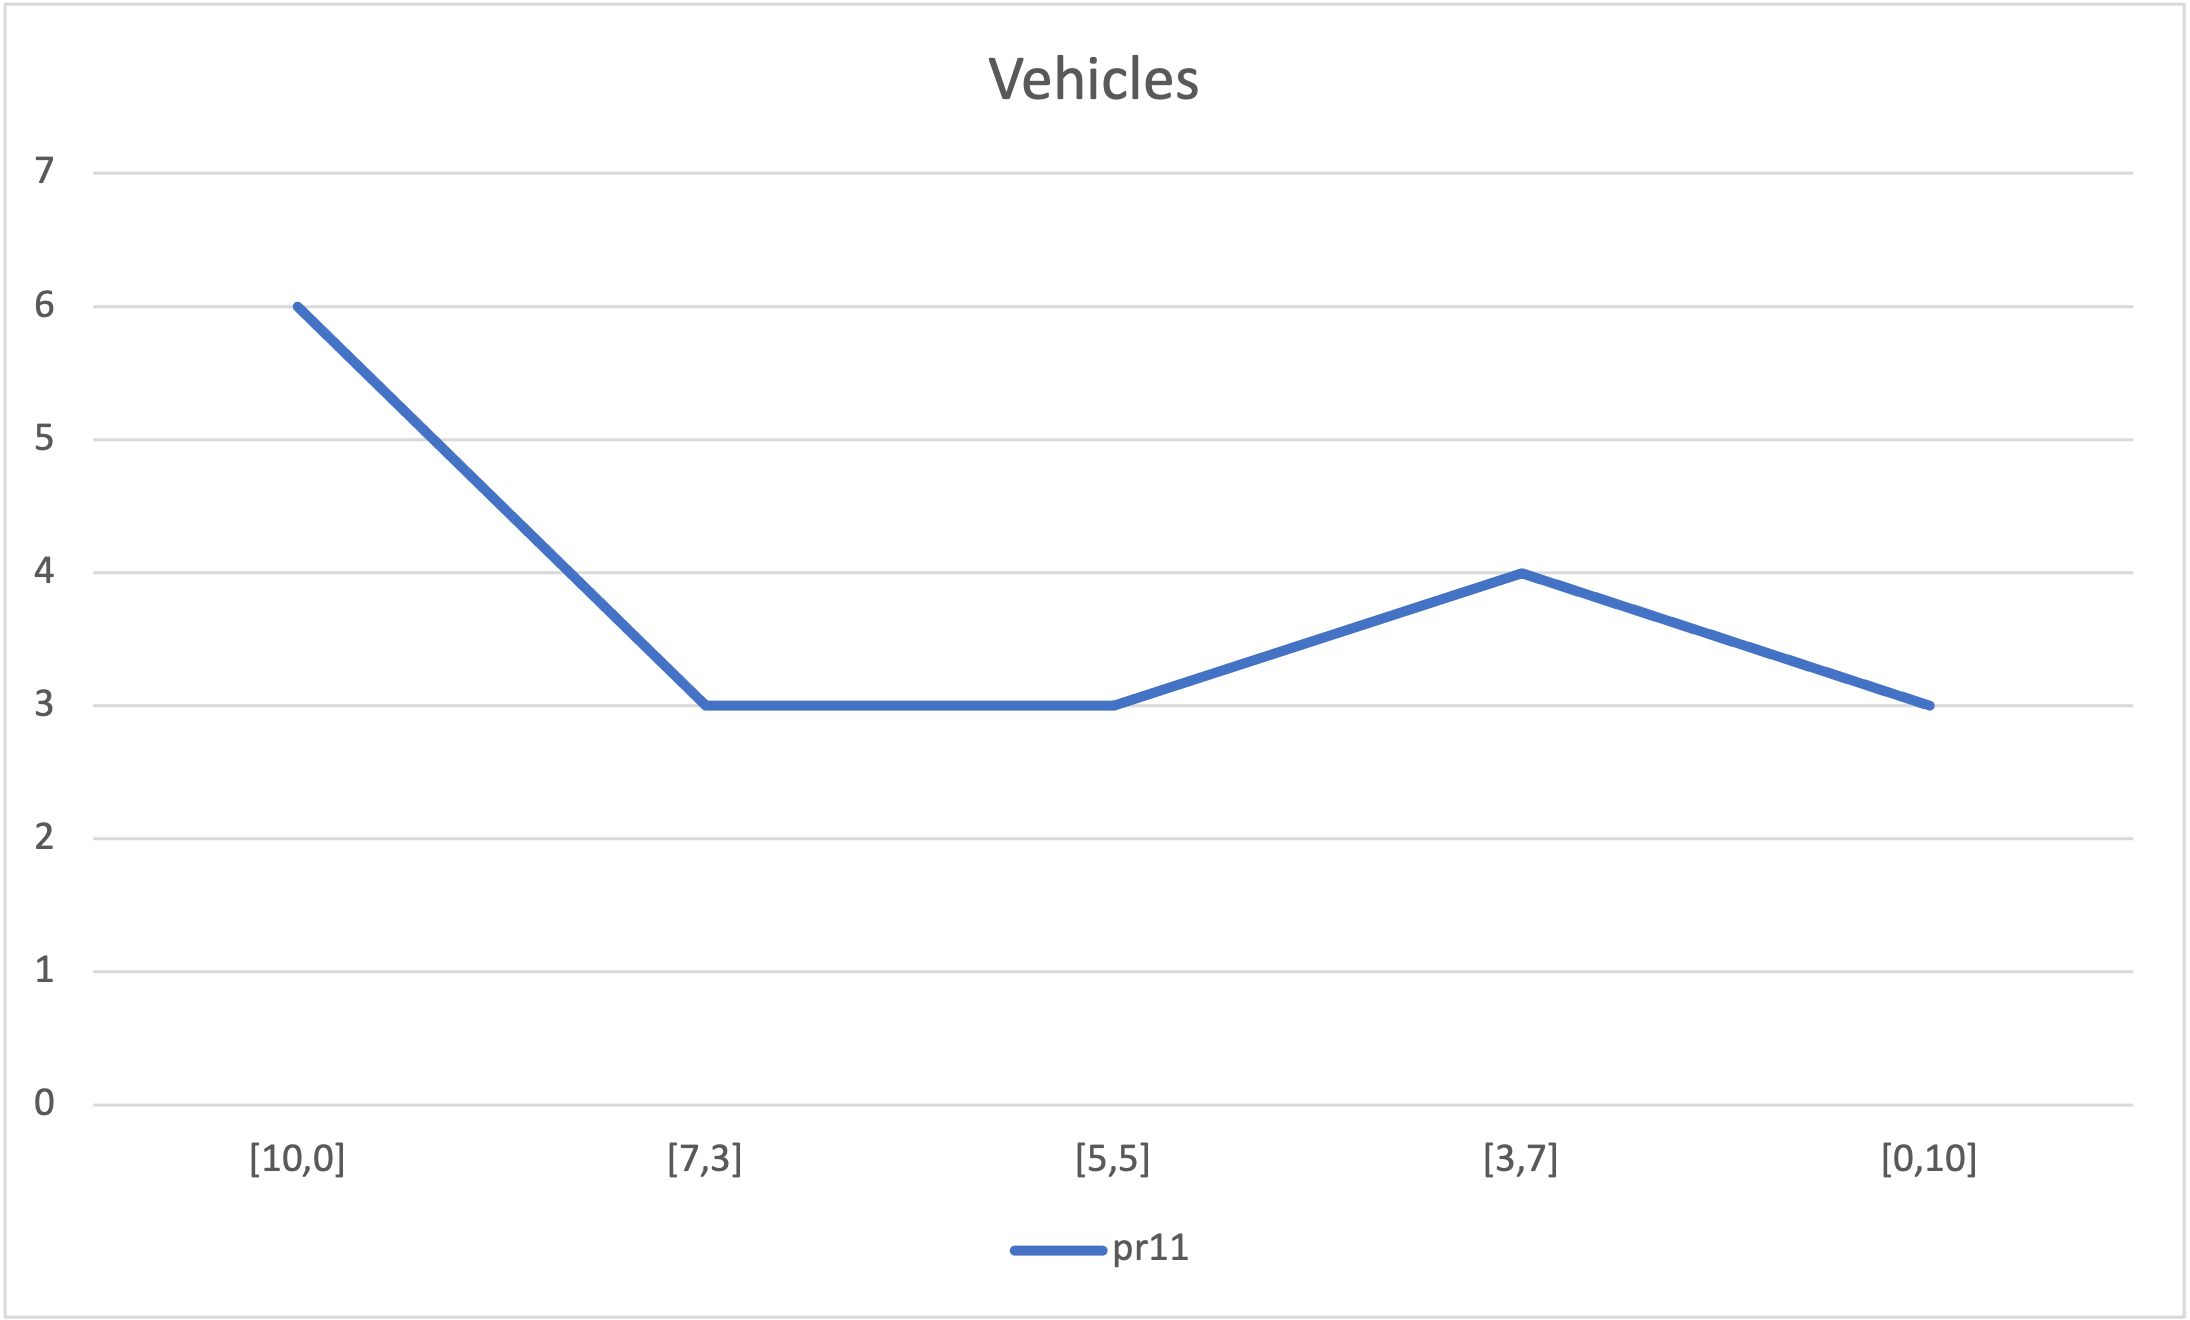
\includegraphics[height=0.25\textheight]{../graphs/pr11-vehicles.png}
    \caption{Vehicles used graph for \textbf{pr11}.}
\end{figure}

\newpage
